\section{Results}
This chapter shows the results of our research methods that we have used.

\subsection{Survey results}
From our survey form, we received 47 results, with all questions completed. We converted the data returned to us to a CSV (Comma-separated values) file and imported it into RStudio, as we did not want the data visualized by Google itself. From our survey we took the questions that we found the most useful and visualized them into plots. 
\begin{figure}[H]
	\centering
	\textbf{\caption{Question: What type of network do you use for playing games?}}
	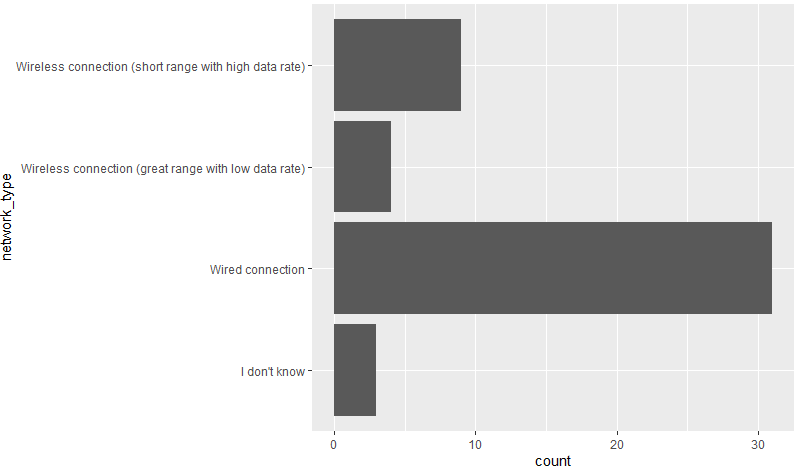
\includegraphics[width=12cm]{../img/network.png}
	
\end{figure}

The barplot shows that most people make use of a wired connection when they play games, where a few people use a wireless connection with either a great range (low data rate) or short range (high data rate). What was alos included in this survey was the question what system the interviewee uses to play video games, the most picked option was Windows/Microsoft. Which makes sense why the wired connection has been picked the most from this question, since wired connection is the most preferred connection type for PC gaming.

\begin{figure}[H]
	\centering
	\textbf{\caption{Question: Do you have a strong internet connection?}}
	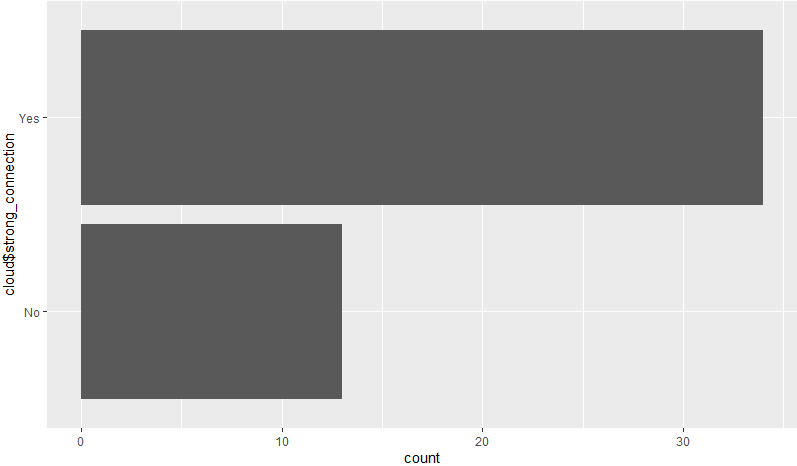
\includegraphics[width=12cm]{../img/connection.png}

\end{figure}

As shown in the chart above, most people claimed that they have a strong Internet connection, while a few people claimed that they do not have a strong Internet connection. We claimed from this that those who had chosen the option "No", that they use a wireless connection and the rest chose the option "Yes" because of a wired connection.

\begin{figure}[H]
	\centering
	\textbf{\caption{Question: When you play an online game, do you often have latency issues?}}
	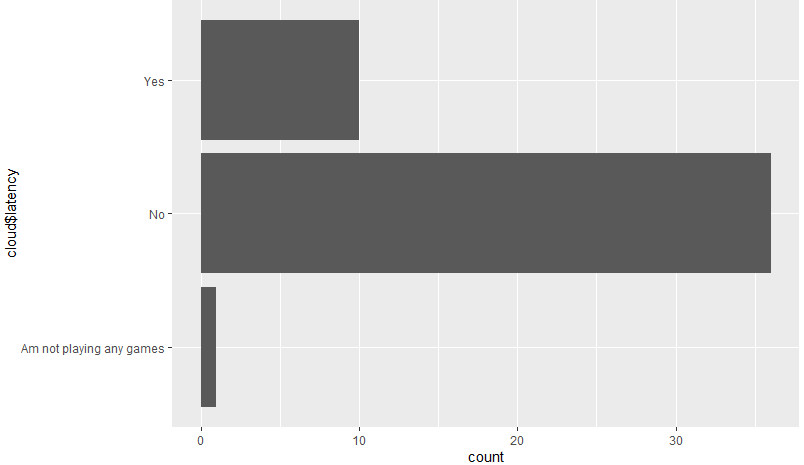
\includegraphics[width=12cm]{../img/latency.png}

\end{figure}

Most people said that they don't often experience latency/lag issues when they play an online game, but a few do experience latency. The people that answered "No" are most likely users of a wired internet connection, whereas the people that have said "Yes" are using a wireless connection.

\begin{figure}[H]
	\centering
	\textbf{\caption{Question: How interested are you in cloud gaming?}}
	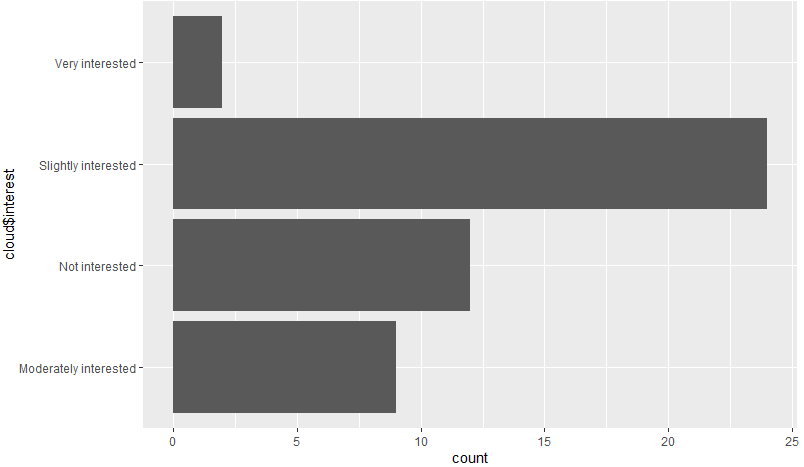
\includegraphics[width=12cm]{../img/interest.png}
	
\end{figure}

People had the choice to fill in how interested they are in cloud gaming. Most people have said that they are slightly interested in it. \\\textbf{From high to low:}\\\\
	Super interested\\
	Very interested\\
	Moderately interested\\
	Slightly interested\\
	Not interested\\\\
In the survey, we also had questions that were about the use of cloud gaming and what the respondents thought of it, such as: For cloud gaming you are attached to a monthly fee between 10 and 60 euros, that in cloud gaming you stream your games from a data center and not at home and that you require a strong and stable internet connection to make the best use of cloud gaming. Most interviewees had mixed thoughts about cloud gaming, which could have affected the question about the interest, having it mixed results. Half of all respondents gave it slight interest and a quarter chose to have no interest in it.

\begin{figure}[H]
	\centering
	\textbf{\caption{Question: Do you think cloud gaming has a future?}}
	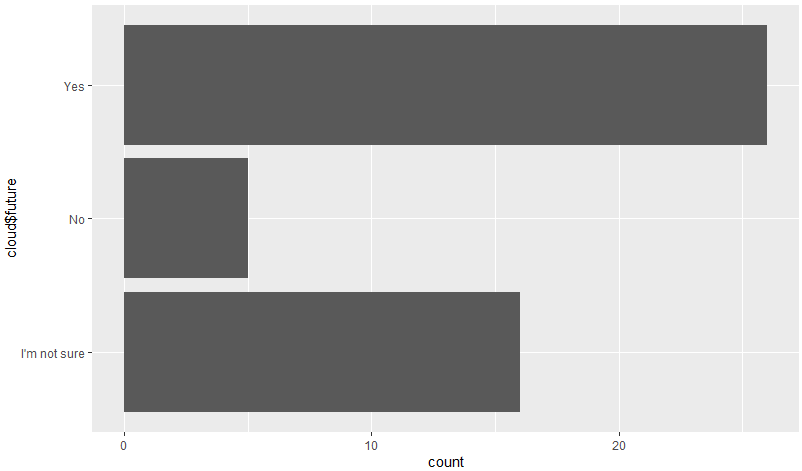
\includegraphics[width=12cm]{../img/future.png}

\end{figure}

For this question, respondents could answer whether cloud gaming has a future for video games. They could choose "Yes", "No" or "I'm not sure". Although there were mixed interests in cloud gaming, many believed that cloud gaming could have a future for video games, in which some did not believe in it, or were unsure about it

\begin{figure}[H]
	\centering
	\textbf{\caption{Question: How likely are you going to give cloud gaming a try?}}
	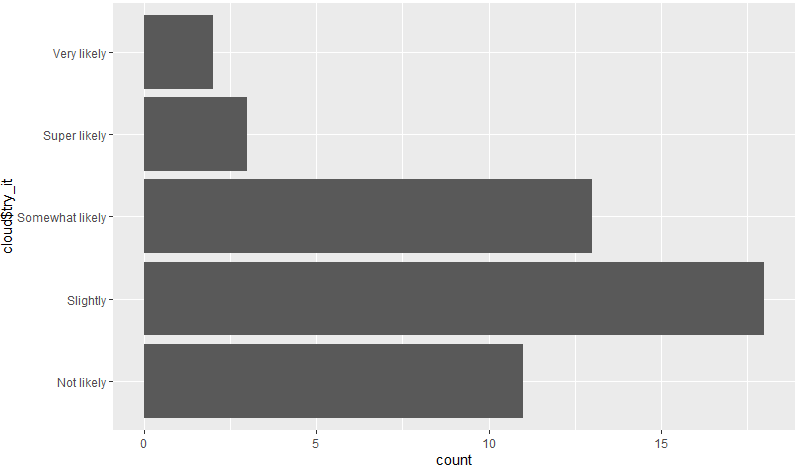
\includegraphics[width=12cm]{../img/try.png}
\end{figure}

Just like the question about how interested people were in cloud gaming, for this question people had the choice to fill in how likely they want to give cloud gaming a try. \\\textbf{From high to low:}\\\\
	Super likely\\
	Very likely\\
	Somewhat likely\\
	Slightly\\
	Not likely\\
	
This question was considered redundant by some interviewees. This could be true because the question about interest in cloud gaming was quite similar, only our thinking on this question was different. We saw this question as literally "Are you ever going to try cloud gaming?", but was changed to "How likely is it that you will try cloud gaming?", and most saw this as an unnecessary question because they had previously indicated whether they were interested in cloud gaming. In which the most frequently chosen option was "Slightly", as with the question about interest.
\\
\subsection{Research methods from articles}

We have come across a number of research articles related to cloud gaming, latency, and latency occurring in cloud gaming. Many articles used methods where they let people play in a cloud gaming environment and add an additional level of latency, to find out how people performed with the game that they were playing. 
\\\\
In the year 2020, "\citeauthor{desveaux2020effects}" performed a research about the effects of latency in commercial cloud gaming services. According to their Background and Related Work \parencite[Chapter 2.3, Page 17]{desveaux2020effects} increased latency generally has a negative impace on both player performance and Quality of Experience, whereby they wanted to conduct a similar experiment with it, by letting someone play Assassin's Creed Odyssey via different cloud gaming services with increased latency \parencite[Chapter 3, Page 18]{desveaux2020effects}.\\
After the experiment, "\citeauthor{desveaux2020effects}" collected the data into two separate types, subjective and objective data. For the subjective data \parencite[Chapter 4.2.2, Page 36]{desveaux2020effects}, the participants were asked to rate the graphics quality, responiveness of the controls and their willingness to continue playing under a certain added latency value.
\begin{figure}[H]
	\centering
	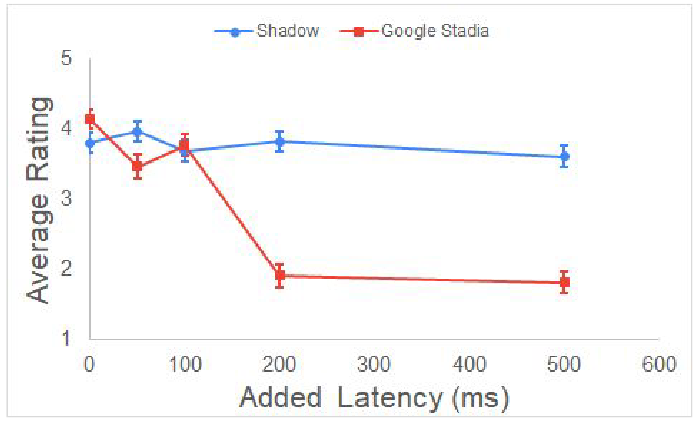
\includegraphics[width=12cm]{../img/fig13.png}
	\caption{Average Rating vs Added Latency for Graphics Quality}
	\parencite[Chapter 4.2.2, Page 36, Figure 13]{desveaux2020effects}
\end{figure}
\begin{figure}[H]
	\centering
	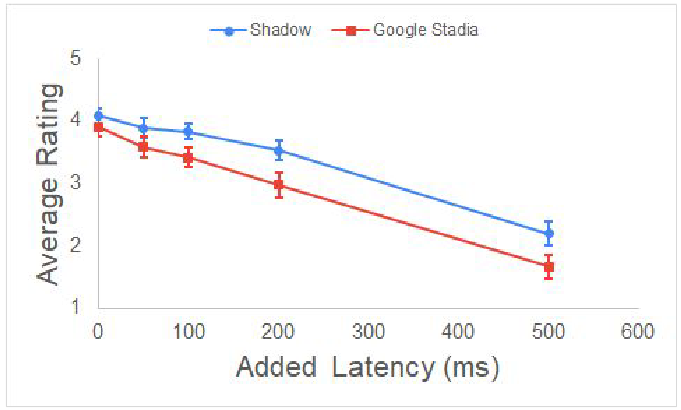
\includegraphics[width=12cm]{../img/fig14.png}
	\caption{Average Rating vs Added Latency for Responsiveness}
	\parencite[Chapter 4.2.2, Page 37, Figure 14]{desveaux2020effects}
\end{figure}
\begin{figure}[H]
	\centering
	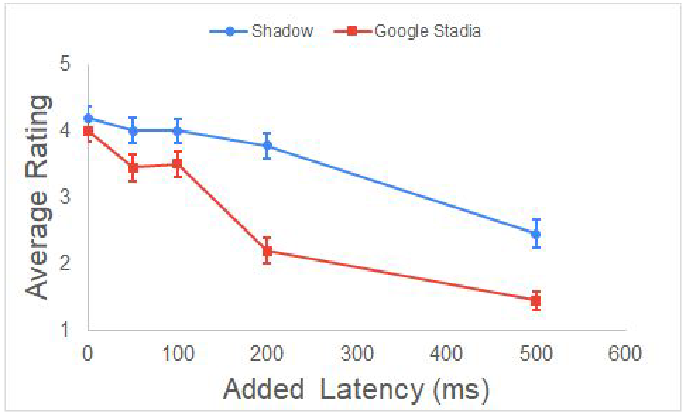
\includegraphics[width=12cm]{../img/fig15.png}
	\caption{Average Rating vs Added Latency for Willingness to play again}
	\parencite[Chapter 4.2.2, Page 37, Figure 15]{desveaux2020effects}
\end{figure}
The objective data \parencite[Chapter 4.2.3, Page 39]{desveaux2020effects} included the number of enemy kills as well as the number of times the participants were hit by enemy attacks.
\begin{figure}[H]
	\centering
	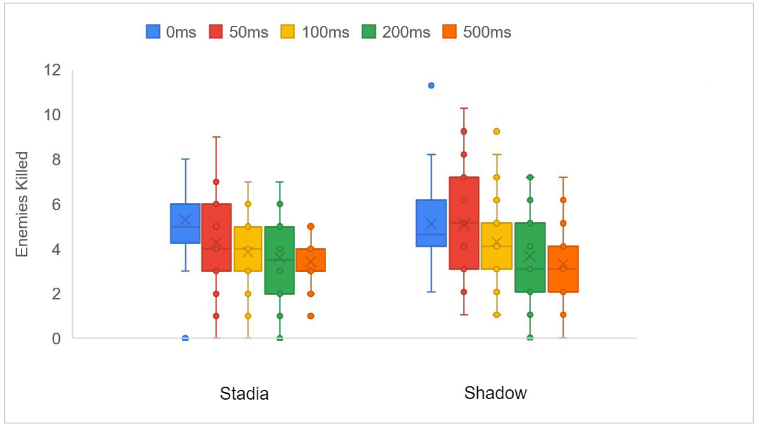
\includegraphics[width=12cm]{../img/fig16.png}
	\caption{Average Number of Enemies Killed for Various Added Latencies}
	In both services, the number of kills went downward as latency increased.\\
	\parencite[Chapter 4.2.3, Page 40, Figure 16]{desveaux2020effects}
\end{figure}
\begin{figure}[H]
	\centering
	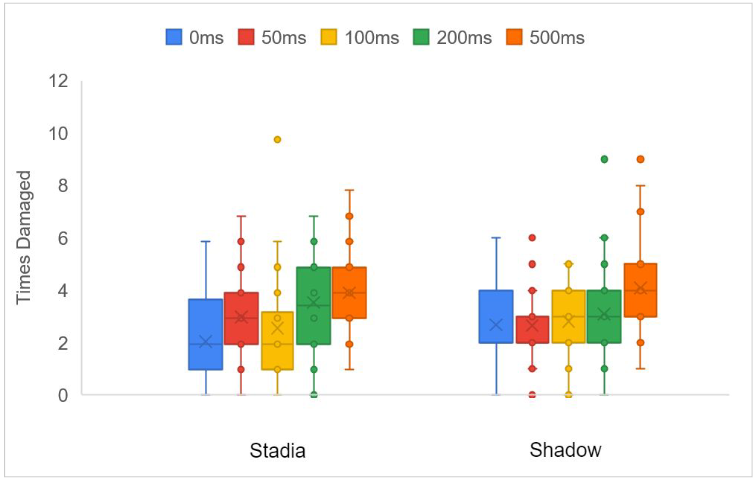
\includegraphics[width=12cm]{../img/fig17.png}
	\caption{Average Number of Times Damaged for Various Different Added Latencies}
	\parencite[Chapter 4.2.3, Page 40, Figure 17]{desveaux2020effects}
\end{figure}
\begin{figure}[H]
	\centering
	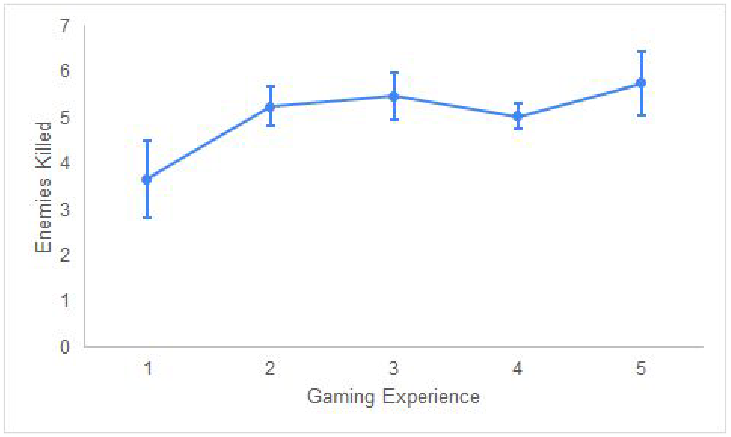
\includegraphics[width=12cm]{../img/fig18.png}
	\caption{Average Enemies Killed by Self Rated Gaming Experience}
	Number of kills went slightly upward depending on the gaming experience.\\
	\parencite[Chapter 4.2.3, Page 41, Figure 18]{desveaux2020effects}
\end{figure}
\begin{figure}[H]
	\centering
	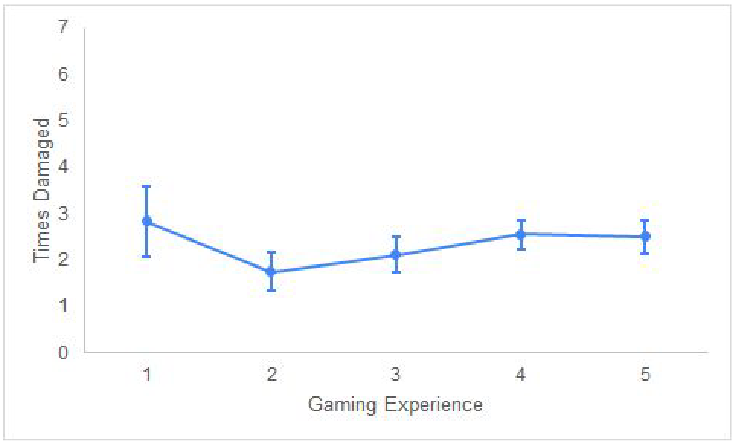
\includegraphics[width=12cm]{../img/fig19.png}
	\caption{Average Times Damaged by Self Rated Gaming Experience}
	\parencite[Chapter 4.2.3, Page 41, Figure 19]{desveaux2020effects}
\end{figure}
\newpage
"\textcite{claypool2014effects}" performed a somewhat similar experiment where people play the game Crazy Taxi and Neverball on the cloud gaming services OnLive and GamingAnywhere \parencite[Chapter 3]{claypool2014effects}. In the game Crazy Taxi the player needs to earn points by driving a cab and transport as many customers to their destinations as quick as possible. Extra points can be earned by performing stunts with the cab \parencite[Chapter 3.A]{claypool2014effects}. In Neverball the player controls a stage level with a marble in it, the player needs to move the marble to its destination as fast as possible by tilting the stage with the arrow keys \parencite[Chapter 3.A]{claypool2014effects}. This experiment was done on older cloud gaming services.
\begin{figure}[H]
	\centering
	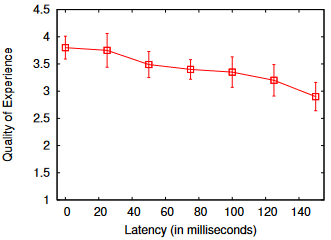
\includegraphics[width=12cm]{../img/fig20.png}
	\caption{QoE for Crazy Taxi on OnLive versus Latency}
	\parencite[Chapter 4, Figure 4]{claypool2014effects}
\end{figure}
\begin{figure}[H]
	\centering
	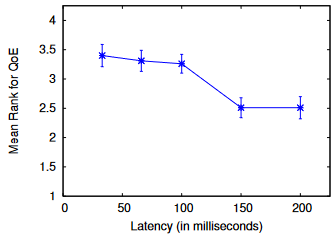
\includegraphics[width=12cm]{../img/fig21.png}
	\caption{QoE for Neverball on GamingAnywhere versus Latency}
	\parencite[Chapter 4, Figure 5]{claypool2014effects}
\end{figure}
\begin{figure}[H]
	\centering
	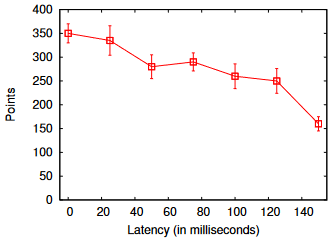
\includegraphics[width=12cm]{../img/fig22.png}
	\caption{User Points for Crazy Taxi on OnLive versus Latency}
	\parencite[Chapter 4, Figure 6]{claypool2014effects}
\end{figure}
\begin{figure}[H]
	\centering
	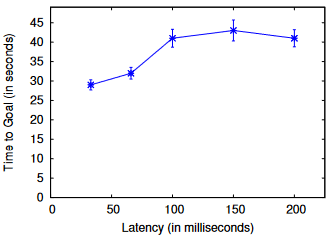
\includegraphics[width=12cm]{../img/fig23.png}
	\caption{User Times for Neverball on GamingAnywhere versus Latency}
	\parencite[Chapter 4, Figure 7]{claypool2014effects}
\end{figure}
\begin{figure}[H]
	\centering
	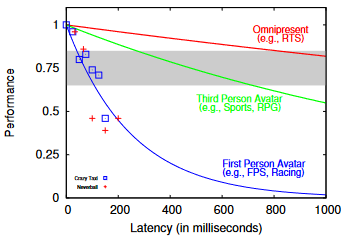
\includegraphics[width=12cm]{../img/fig24.png}
	\caption{User Performance versus Latency for Classes of Games}
	\parencite[Chapter 4, Figure 8]{claypool2014effects}
\end{figure}
"\textcite{anouna2014network}" also performed an experiment with the game Neverball that was using the cloud gaming service GamingAnywhere and used Dummynet to control the latency between the client and server \parencite[Chapter 3.2, Page 6]{anouna2014network}. One level was chosen for this experiment to measure the players' performances by the time it took them to complete the level \parencite[Chapter 4.1, Page 15]{anouna2014network}.
\begin{figure}[H]
	\centering
	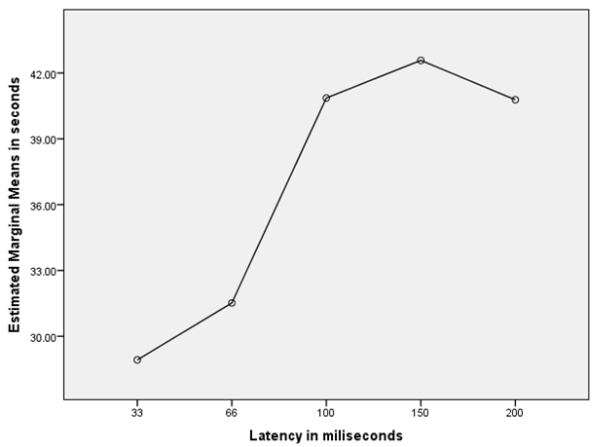
\includegraphics[width=12cm]{../img/fig25.png}
	\caption{A graph of the average time to complete at each latency}
	\parencite[Chapter 4.1, Page 15, Figure 4.1]{claypool2014effects}
\end{figure}
\newpage
The research article \citetitle{7536162} by "\citeauthor{7536162}" was the final research article we had come around. This research article included theories and methodologies from 100+ articles (as reference) that were related to cloud gaming and latency, which was very beneficial for us to include for our research.\\\\
According to \textcite[Chapter VI]{7536162}, minimizing the cost on cloud and network recources while achieving high gamer experience requires careful optimization. If the careful optimizations are not met, service providers cannot consolidate enough users to each physical machine, which leads to lower profits and may drive the service provider out of business. As new cloud gaming services with better optimization enter the market, more competition follows in the gaming industry. As commercial cloud gaming services become financially sustainable, cloud gaming will continue to expand, leading to more investments and improvements for these services. To push cloud gaming even further in the market may need to create new programming paradigms to support the unique needs of these complex systems. \textcite[Chapter VI]{7536162} summarized that the advances of technologies turns playable cloud gaming services into a reality, where more optimization techniques makes cloud gaming services profitable, making our way to a new era of a new cloud gaming ecosystem, leading to the next generation of cloud gaming services.